% D7 sec6 草稿 v2.1（2026-11-01）, 相对 v2.0 的改动（零新实验, 新增数字都取自冻结的结果文件）:
%   删掉 6.1 里与 §5.3 重复的协议复述, 压成导语段;
%   6.7 新增 holdout 小表（摘要三个 holdout 数字 82%/0.57/95.7% 的正文落点）;
%   全文协议标注补齐（cv10 pooled / holdout）, 表标题均带协议;
%   6.4 统计描述压成两句, 120 对清点移脚注（引 results/ttest/ 的 C5 记录）;
%   记号统一为 "30.0% positives"/"6.1% positives" 这类百分比写法;
%   6.6 开头接收集成 setup 段（自 C 的 §5.4 迁入, 写回时 C 需同步从 sec5 删掉该段）;
%   6.6 末尾加运行成本一句: 84 次运行共 116 s、最贵 sick ada+SMOTE cv10 28.9 s（run_log_v1.csv）;
%   6.5 Missingness 段补插补消融数字（b4_missing_comparison.csv: 插补 0.830±0.049/AUC 0.974
%        vs 删行 0.843±0.069/0.964, n=3772/2643; 标记值 0.828/0.965）。
% 写回 overleaf 时: cp 本文件 overleaf/sections/sec6_results.tex（去注释头）;
%   sec6 与 sec7 要成对写回（6.7 引用 sec7 的 \label{sec:conclusion}）, 写回前先 pull。

\section{Results and Evaluation}
\label{sec:results}
% D 负责本文件: 指标、图、跨数据集对比与统计检验。
% RQ 对应关系见 docs/RQ_定义与映射_v1.0.md（2026-10-29 全组定的版本）— credit-g/sick/显著性
% 三节答 RQ1/RQ2, 跨数据集节兼答 RQ3, holdout 节答 RQ4; 评估协议只在 §5.3 讲一次。

Throughout this section the positive class is \texttt{bad} for credit-g and \texttt{sick} for sick; F1, precision and recall refer to it, and AUC is computed from out-of-fold positive-class probabilities. Threshold-adjusted models selected their threshold $\tau$ on development folds only (observed range 0.20--0.60), and their AUC is bitwise identical to the plain model's --- $\tau$ moves the operating point, not the score ranking. A ZeroR majority-class baseline appears as a reference row in each table, not as a competitor. Every number traces to the archived result files named in the table captions. Sections~\ref{sec:results-creditg}--\ref{sec:results-sig} answer RQ1 (strategy and model selection under imbalance and asymmetric cost) and RQ2 (when accuracy misleads and which metrics should decide); Section~\ref{sec:results-flip} additionally carries the encoding and feature-importance cross-references of RQ3; Section~\ref{sec:results-holdout} answers RQ4 (decision quality on unseen samples).

\subsection{credit-g: Accuracy Is Cheap, Minority Recall Is Not (RQ1)}
\label{sec:results-creditg}

\begin{table}[H]
\centering
\caption{credit-g, cv10 F1 (mean $\pm$ std over 10 folds; positive class \texttt{bad}). Champion in \textbf{bold}. Full metric set: \texttt{results/all\_metrics\_v1.csv}.}
\label{tab:creditg-f1}
\begin{tabular}{lcccc}
\toprule
Model & Plain & SMOTE & Cost-sensitive & Threshold \\
\midrule
Decision Tree & $0.322\pm0.192$ & $0.471\pm0.078$ & $0.523\pm0.030$ & $0.561\pm0.038$ \\
Random Forest & $0.499\pm0.079$ & $0.509\pm0.077$ & $0.595\pm0.064$ & $0.595\pm0.059$ \\
Logistic Reg. & $0.531\pm0.060$ & $0.591\pm0.051$ & $\mathbf{0.597\pm0.034}$ & $0.591\pm0.049$ \\
SVC & $0.498\pm0.101$ & $0.560\pm0.050$ & $0.593\pm0.032$ & $0.590\pm0.055$ \\
\midrule
ZeroR (ref.) & \multicolumn{4}{c}{F1 $=0$ (acc.\ 0.700, recall 0)} \\
\bottomrule
\end{tabular}
\end{table}

Table~\ref{tab:creditg-f1} shows the cv10 F1 landscape. Three observations:

\textbf{(i) Plain models fall into the accuracy trap.} The three plain tree/kernel models (DT, RF, SVC) sit at or below ZeroR-level recall (0.27--0.40), trading minority detection for majority-class accuracy (0.71--0.77); their plain F1 (0.32--0.50) is the worst column. This is the RQ2 pattern: high accuracy is achievable while detecting almost no bad credit.

\textbf{(ii) Every intervention helps here.} All three strategies lift F1 for every model on credit-g (mean $\Delta$F1 $+0.070$ to $+0.122$); the champion is \emph{cost-sensitive logistic regression} (\texttt{lr\_cost}, F1 $0.597\pm0.034$, recall $0.863$ vs.\ $0.470$ plain, precision $0.456$), which applies the official 5:1 misclassification cost as class weights and moves the decision boundary without synthesising data or adding capacity. Its pooled confusion cost $(5\,\mathrm{FN}+\mathrm{FP})/N$ over the cv10 out-of-fold predictions drops to $0.514$ from $0.884$ (plain LR).

\textbf{(iii) The holdout agrees.} On the 70:30 holdout, \texttt{lr\_cost} reaches F1 $0.580$ / recall $0.822$, within one standard deviation of the cv10 estimate --- no setting was tuned on the holdout. Section~\ref{sec:results-holdout} evaluates this as a decision rule (RQ4).

\subsection{sick: Strategies Move the Operating Point, Not the Ranking (RQ1)}
\label{sec:results-sick}

\begin{table}[H]
\centering
\caption{sick, cv10 F1 (mean $\pm$ std; positive class \texttt{sick}). Champion in \textbf{bold}. The cost arm on sick is an equal-cost control (frozen weights $\{1,1\}$: the dataset has no official cost matrix): DT/LR/SVC reproduce plain bitwise; RF differs by one pooled instance (split tie-flip, Section~\ref{sec:results-sick}).}
\label{tab:sick-f1}
\begin{tabular}{lcccc}
\toprule
Model & Plain & SMOTE & Cost-sensitive & Threshold \\
\midrule
Decision Tree & $0.836\pm0.050$ & $0.747\pm0.050$ & $0.836\pm0.050$ & $0.820\pm0.048$ \\
Random Forest & $0.870\pm0.047$ & $\mathbf{0.897\pm0.051}$ & $0.873\pm0.048$ & $0.877\pm0.052$ \\
Logistic Reg. & $0.687\pm0.091$ & $0.521\pm0.028$ & $0.687\pm0.091$ & $0.745\pm0.038$ \\
SVC & $0.763\pm0.064$ & $0.742\pm0.039$ & $0.763\pm0.064$ & $0.809\pm0.039$ \\
\midrule
ZeroR (ref.) & \multicolumn{4}{c}{F1 $=0$ (acc.\ 0.939, recall 0)} \\
\bottomrule
\end{tabular}
\end{table}

The sick landscape differs structurally from credit-g. First, \textbf{SMOTE hurts the models it should help}: it is the only strategy that reduces F1 for DT ($-0.089$, $p=0.048$) and collapses logistic regression ($-0.166$, $p=0.002$), while leaving Random Forest intact ($+0.027$, n.s.). Second, \textbf{the cost arm on sick is by design an equal-cost control}: the dataset has no official cost matrix, so the frozen specification sets the class weights to $\{1,1\}$ and expects the result to reproduce plain as a sanity check --- which it does bitwise for DT, LR, and SVC (pooled confusion matrices identical, $\Delta=0$, $p=1$). Random Forest alone deviates, by a single pooled instance (FN $44\to43$): a tie-flip that explicitly weighted tree splits are known to produce, recorded in the test ledger and not interpreted as a strategy effect. The genuine cost intervention is the credit-g arm, which carries the official 5:1 weights (Section~\ref{sec:results-creditg}). Third, Figure~\ref{fig:rocpr} shows the three strategies' ROC and PR curves nearly coincide (AUC $0.997$--$0.998$ for Random Forest): the interventions move the \emph{operating point}, not the score ranking, so their entire effect is a precision--recall trade along an essentially fixed curve.

\begin{figure}[H]
\centering
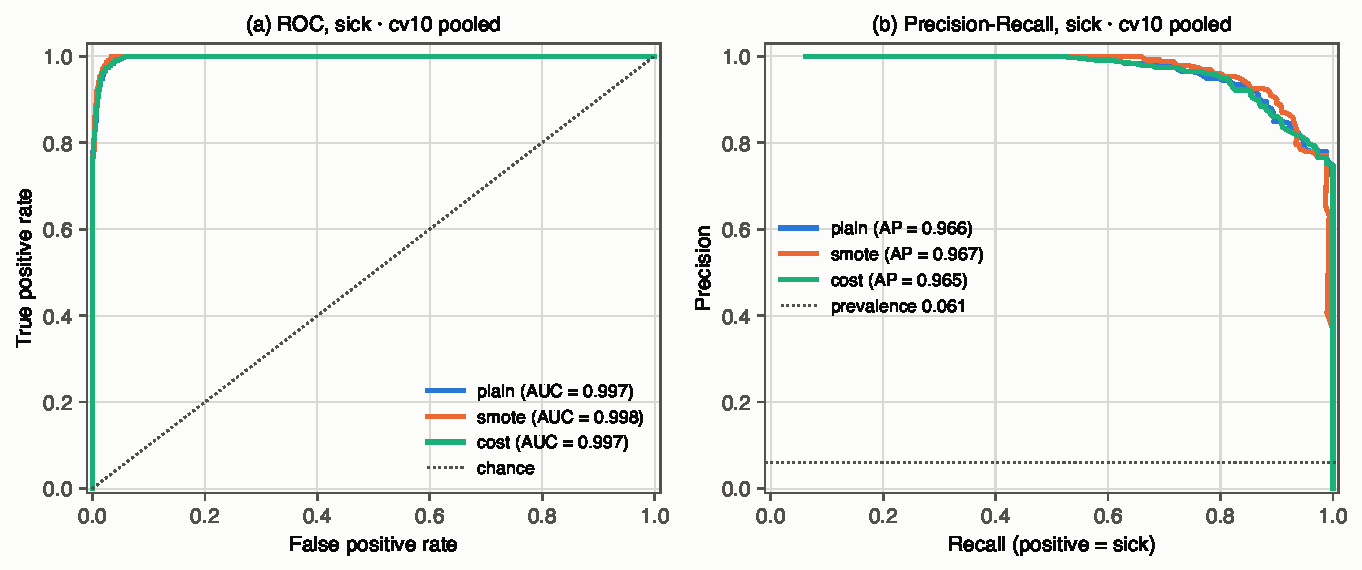
\includegraphics[width=\textwidth]{figures/fig_d_sick_roc_pr.pdf}
\caption{ROC (a) and Precision--Recall (b) curves on sick for Random Forest under plain, SMOTE, and cost-sensitive strategies, computed from pooled out-of-fold predictions of the 10-fold cross-validation protocol (all 3{,}772 instances; positive class \texttt{sick}). Dotted lines mark chance level (a) and the positive-class prevalence $231/3772=0.061$ (b). The curves nearly coincide: ranking quality is strategy-invariant. Source data: \texttt{results/preds/sick\_rf\_*\_v1\_run1\_cv10\_preds.csv}.}
\label{fig:rocpr}
\end{figure}

\subsection{Strategy Effects and Statistical Significance (RQ1, RQ2)}
\label{sec:results-sig}

\begin{figure}[H]
\centering
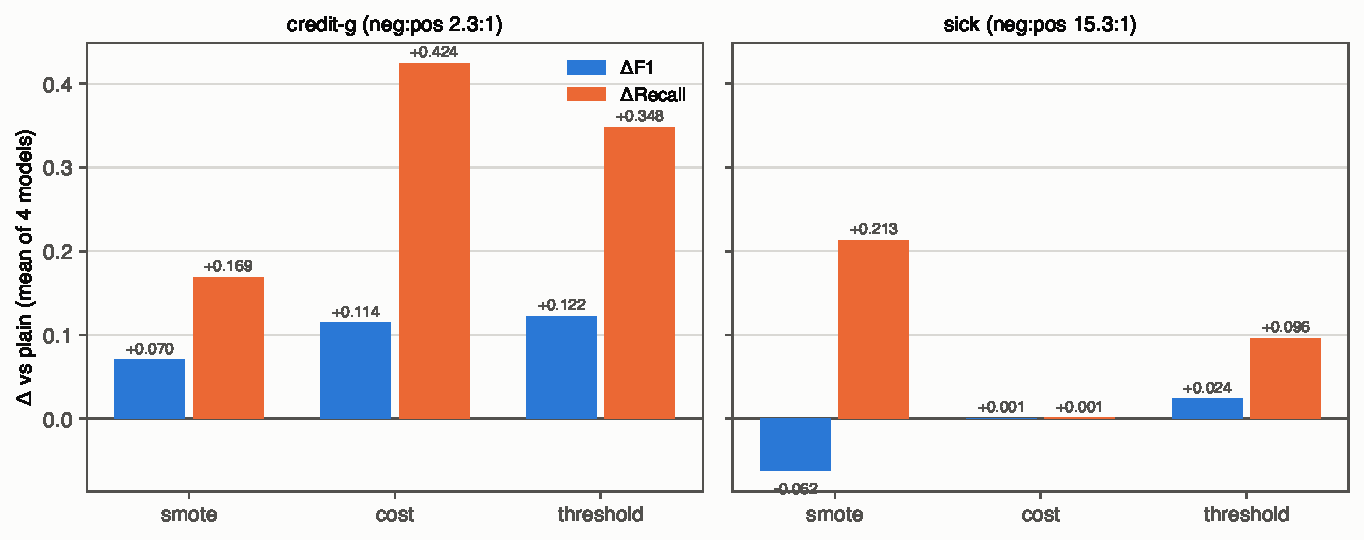
\includegraphics[width=\textwidth]{figures/fig_d_strategy_gain.pdf}
\caption{Effect of each imbalance-handling strategy relative to plain training, averaged over the four base models (cv10): $\Delta$F1 (blue) and $\Delta$Recall (orange), $\Delta=$ strategy $-$ plain, from the twelve pre-specified paired comparisons per metric (Nadeau--Bengio corrected $t$-tests). Left: credit-g (positive \texttt{bad}, 30.0\% positives); right: sick (positive \texttt{sick}, 6.1\% positives). Recall gains are non-negative everywhere while F1 gains flip sign on sick. Source: \texttt{results/cross\_dataset\_comparison\_v1.csv}.}
\label{fig:gain}
\end{figure}

For RQ2, the failure of accuracy is a pre-registered finding, not a post hoc observation: the accuracy-trap rule (accuracy $\geq 0.70$ and recall $\leq 0.40$, fixed before evaluation) flags ten archived units --- all four ZeroR reference cells and six of the eight plain credit-g cells (DT, RF, SVC under both protocols; the RF cv10 cell sits exactly on the 0.40 recall boundary, and LR, at recall 0.47--0.48, is the only plain model above it). No plain sick cell qualifies, because sick's minority is nearly separable (RF AUC 0.998) and even plain models detect it: the trap binds when the minority is both small and hard to rank, as on credit-g.

Twelve pre-specified strategy-vs-plain comparisons per metric were tested with fold-level paired $t$-tests corrected for fold overlap following Nadeau and Bengio (variance factor $0.2111$, i.e.\ $2.11\times$ the naive variance --- deliberately conservative); stars denote raw $p$ at $\alpha=0.05$ ($^{*}<0.05$, $^{**}<0.01$, $^{***}<0.001$). Under Holm correction within each metric family the outcome splits cleanly: none of the twelve pre-specified F1 contrasts survives, whereas eight of the twelve recall contrasts do (all cost/threshold) --- the strategies reliably buy recall, and it is the precision price that depends on the dataset.\footnote{Full counting over all 120 pairwise contrasts per family is archived in the test run ledger (\texttt{results/ttest/}, document C5): on credit-g exactly one pair of 120 survives Holm (\texttt{dt\_smote} vs \texttt{lr\_smote}, $p_{\mathrm{Holm}}=0.021$); on sick 22 pairs survive, almost all of the form ``every configuration beats the collapsed \texttt{lr\_smote}/\texttt{svc\_smote}''.} Figure~\ref{fig:gain} summarises the pre-specified pattern:

\begin{itemize}
  \item \textbf{Recall gains are same-direction everywhere}: all twelve comparisons raise recall (credit-g $+0.06$ to $+0.59$, sick $+0.004$ to $+0.28$), nine significantly.
  \item \textbf{F1 gains flip across datasets}: three sign flips on sick (DT and LR $\times$ SMOTE, DT $\times$ threshold), all concentrated in SMOTE$\times$(DT/LR). The strategies reliably buy recall; the precision price is what depends on the dataset.
  \item \textbf{Accuracy drops almost everywhere} (credit-g cost/threshold $-0.04$ to $-0.19$, mostly significant; sick $\leq 0.07$): minority gains are paid for in majority-class accuracy, and accuracy alone would have hidden them.
\end{itemize}

\subsection{Cross-Dataset Comparison: The Winner Flips (RQ1; RQ3 Cross-References)}
\label{sec:results-flip}

\begin{figure}[H]
\centering
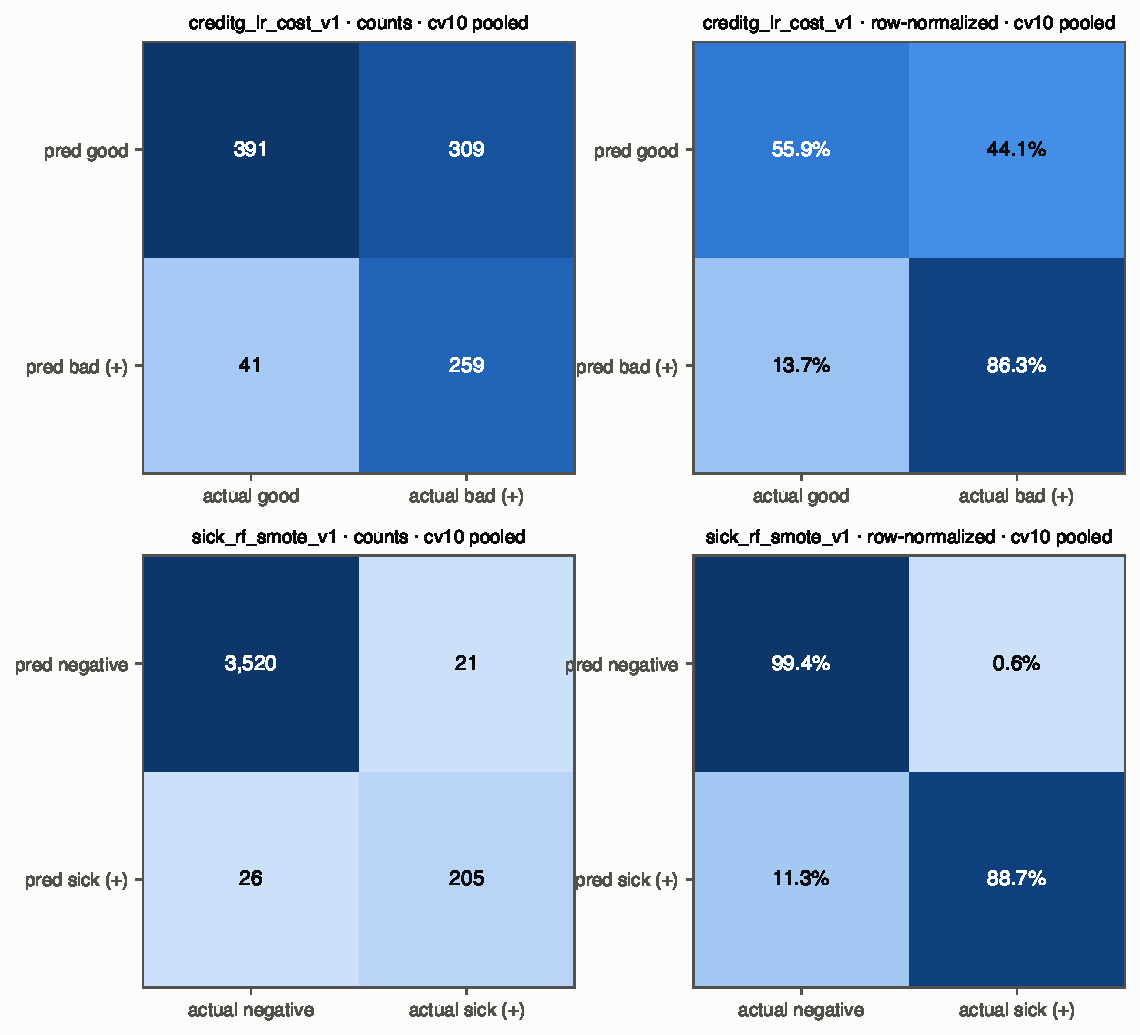
\includegraphics[width=0.8\textwidth]{figures/fig_d_confusion.pdf}
\caption{Confusion matrices of the per-dataset F1 champions (cv10, pooled out-of-fold predictions; rows = predicted, columns = actual; $(+)$ marks the positive class): credit-g \texttt{lr\_cost} (top, positive \texttt{bad}) and sick \texttt{rf\_smote} (bottom, positive \texttt{sick}). Left: counts; right: row-normalised. Source: \texttt{results/all\_metrics\_v1.csv}.}
\label{fig:confusion}
\end{figure}

The two datasets crown different winners (Figure~\ref{fig:confusion}): credit-g rewards \emph{linear + cost-sensitive} (\texttt{lr\_cost}, F1 $0.597$, recall $0.863$, precision $0.456$ --- it catches 259 of 300 bad cases but flags 309 of 700 good ones), while sick rewards \emph{ensemble + resampling} (\texttt{rf\_smote}, F1 $0.897$, recall $0.888$, precision $0.910$ --- near-clean on both error types). A naive single-variable reading --- ``more imbalance needs more resampling'' --- predicts SMOTE should help \emph{more} on sick (6.1\% positives) than on credit-g (30.0\%); the data say the opposite. Four dataset properties jointly explain the flip:

\textbf{Size (1{,}000 vs 3{,}772 rows).} On credit-g, high-capacity learners (RF, AdaBoost, $n_{\mathrm{estimators}}=100$) train on only 900 rows per fold and their variance dominates; a strong-prior linear model plus an intervention that only re-weights the loss (cost) is the stable choice. On sick, capacity pays: bagging reduces variance and boosting reduces bias on 3{,}395-row training folds.

\textbf{Attribute composition (13 vs 22 categorical attributes).} SMOTE interpolates linearly in the one-hot-encoded space, synthesising fractional categories (``half-open door''); sick's sparser one-hot space amplifies this interpolation noise. The linear decision surface of LR is most sensitive (F1 $-0.166$, $p=0.002^{**}$), whereas axis-parallel tree splits depend only on feature ordering and are insensitive (RF $+0.027$, n.s.). The frozen encoding ablation pins down the encoding half of this mechanism on credit-g (RQ3): LR under the one-hot branch (61 features) reaches F1 $0.531$ / AUC $0.785$, against $0.406$ / $0.738$ under ordinal codes (20 features; fold-level paired $p=0.021$ / $0.008$), and the ordinal branch fails to converge within its 1{,}000-iteration budget where the one-hot branch converges in 55; an attribution control (ordinal codes with standardised numerics, F1 $0.415$) stays next to the ordinal branch, isolating encoding --- not scaling --- as the cause (Section~\ref{sec:data}). Feature-importance triangulation agrees on \emph{which} fields matter: the random forest's top three attributes (credit\_amount $0.141$, duration $0.107$, checking\_status $0.107$) supply the same fields as the strongest Apriori rule (duration in its top quintile together with savings below 100 implies \texttt{bad} at 57.3\% confidence against a 30\% base rate, lift 1.91; Section~\ref{sec:apriori}).

\textbf{Missingness (0\% vs 29.9\% of rows).} sick's imputation noise further penalises distance- and hyperplane-based learners (LR, SVC), while tree ensembles are rank-robust to it --- widening the tree-vs-linear gap that the champion comparison shows. The frozen imputation ablation quantifies the preprocessing side: mean/mode imputation keeps all 3{,}772 rows at F1 $0.830\pm0.049$ / AUC $0.974$, whereas deleting the 1{,}129 incomplete rows (29.9\% of the data, including 19 of the 231 positives) shifts F1 only to $0.843\pm0.069$ --- within one standard deviation --- while AUC falls to $0.964$ (treating missingness as a marker value: F1 $0.828$, AUC $0.965$); rows are therefore kept and imputed within folds (Section~\ref{sec:data}).

\textbf{Imbalance (30.0\% vs 6.1\% positives; neg:pos 2.3:1 vs 15.3:1).} Imbalance explains \emph{strategy choice}, not model choice: at 30\% positives, class weighting suffices to move many boundary cases (recall $+0.34$ to $+0.59^{***}$); at 6.1\% positives, recall must instead be bought by explicit synthesis (SMOTE) or iterative re-weighting (boosting) --- the equal-cost control of Section~\ref{sec:results-sick} has nothing to move on sick, and the official 5:1 weights exist only for credit-g.

In short: small, complete, moderately imbalanced credit-g rewards \emph{correct priors + cost sensitivity}; large, noisy, extremely imbalanced sick rewards \emph{capacity + resampling}. No single dimension predicts the winner.

\subsection{Ensemble Study (Exploratory; RQ1 Supplementary)}
\label{sec:results-ensemble}

As an exploratory extension outside the pre-registered main matrix, bagging (BaggingClassifier) and AdaBoost were run $\times$ \{plain, SMOTE\} $\times$ both datasets, reusing the locked cross-validation splits and the unified evaluation pipeline of the main matrix; both locked protocols were run, and the results are stored in a separate namespace and excluded from the main statistical family. Only two comparisons were pre-specified; the remaining cells are descriptive mean $\pm$ std only (Table~\ref{tab:ensemble} reports cv10).

\begin{table}[H]
\centering
\caption{Ensemble study (exploratory), cv10 (mean $\pm$ std over 10 folds). F1 for the positive class; best exploratory F1 per dataset in \textbf{bold}. Ensemble models are not part of the main matrix or its statistical family. Source: \texttt{results/ensemble\_metrics\_v1.csv}.}
\label{tab:ensemble}
\begin{tabular}{llcccc}
\toprule
Dataset & Config & F1 & Recall & AUC & Runtime (s) \\
\midrule
credit-g & bag+plain & $0.510\pm0.072$ & 0.430 & 0.782 & 2.2 \\
credit-g & bag+SMOTE & $0.548\pm0.074$ & 0.560 & 0.770 & 1.2 \\
credit-g & ada+plain & $0.499\pm0.070$ & 0.473 & 0.735 & 1.2 \\
credit-g & ada+SMOTE & $0.501\pm0.087$ & 0.483 & 0.723 & 2.4 \\
\midrule
sick & bag+plain & $0.819\pm0.050$ & 0.775 & 0.990 & 3.6 \\
sick & bag+SMOTE & $0.785\pm0.037$ & 0.987 & 0.994 & 4.6 \\
sick & ada+plain & $0.918\pm0.045$ & 0.901 & 0.999 & 9.5 \\
sick & ada+SMOTE & $\mathbf{0.937\pm0.043}$ & 0.931 & 0.999 & 28.9 \\
\bottomrule
\end{tabular}
\end{table}

The two pre-specified tests (Nadeau--Bengio corrected, as above) were \texttt{bag\_plain} vs \texttt{dt\_plain} (does bagging reduce the single-tree's variance?) and \texttt{ada\_plain} vs \texttt{dt\_smote} (does boosting's re-weighting substitute for resampling?):

\begin{itemize}
  \item \texttt{bag\_plain} vs \texttt{dt\_plain}: credit-g $+0.188$, $p=0.071$ (n.s.); sick $-0.018$, $p=0.067$ (n.s.).
  \item \texttt{ada\_plain} vs \texttt{dt\_smote}: credit-g $+0.028$, $p=0.389$ (n.s.); \textbf{sick $+0.171$, $p=6.4\times10^{-4***}$}.
\end{itemize}

The one significant result: on sick, boosting's iterative re-weighting significantly outperforms SMOTE resampling at the same base learner --- consistent with \texttt{ada\_smote} posting the highest sick F1 of the whole project ($0.937$). We note that \texttt{ada\_smote} ($0.937$) vs main-matrix champion \texttt{rf\_smote} ($0.897$) was \emph{not} a tested comparison and is descriptive only.

Two zero-cost insights follow from reading Table~\ref{tab:ensemble} against the main matrix, with no additional experiments:

\textbf{(1) Why tree ensembles absorb SMOTE.} \texttt{bag+SMOTE} on sick pushes recall to $0.987$ but F1 \emph{drops} to $0.785$ (precision collapses), while \texttt{ada+SMOTE} converts the same resampled data into balanced gains ($0.931$ recall, $0.943$ implied precision). Combined with the main-matrix finding that SMOTE leaves RF intact but hurts LR, this supports the axis-parallel-split explanation: tree ensembles are robust to one-hot interpolation noise, and boosting additionally re-weights the noisy synthetic minority examples down over rounds instead of trusting them equally.

\textbf{(2) Why the bag/ada ranking flips with the dataset.} On credit-g both ensembles trail the main champion (\texttt{lr\_cost} $0.597$) --- with 900-row training folds, added capacity overfits; on sick both lead every single model --- with 3{,}395-row folds, capacity compounds with resampling. The ensemble flip mirrors the main-matrix winner flip and reinforces the size/attribution story of Section~\ref{sec:results-flip}.

The full study is computationally modest: the archived run log records 84 runs totalling 116 seconds of fit time, the single most expensive being sick \texttt{ada+SMOTE} under cv10 ($28.9$\,s, Table~\ref{tab:ensemble}) --- the entire matrix reproduces on a laptop in minutes.

\subsection{Decision Quality on Unseen Samples (RQ4)}
\label{sec:results-holdout}

Both locked hold-out sets were scored exactly once, after all settings were frozen, on data that never entered training, imputation fitting, or threshold selection (Table~\ref{tab:holdout}). The question here is not ranking quality but decision quality (RQ4): do the per-dataset champions make defensible calls on genuinely new cases?

\begin{table}[H]
\centering
\caption{Locked hold-out performance of the per-dataset champions (RQ4): evaluated once on the unseen 70:30 split (300 credit applicants, 90 \texttt{bad}; 1{,}132 patients, 69 \texttt{sick}) after all settings were frozen. Cost is the official credit-g matrix $(5\,\mathrm{FN}+\mathrm{FP})/N$; sick has no official cost matrix. Source: \texttt{results/all\_metrics\_v1.csv} (holdout rows).}
\label{tab:holdout}
\begin{tabular}{llcccc c}
\toprule
Dataset & Champion & $n$ (pos.) & Recall & Precision & F1 & Cost \\
\midrule
credit-g & \texttt{lr\_cost} & 300 (90) & 0.822 & 0.448 & $\mathbf{0.580}$ & $\mathbf{0.570}$ \\
sick & \texttt{rf\_smote} & 1{,}132 (69) & 0.957 & 0.868 & $\mathbf{0.910}$ & --- \\
\bottomrule
\end{tabular}
\end{table}

\textbf{credit-g: loss control.} The pre-registered champion \texttt{lr\_cost} catches 74 of the 90 bad applicants while flagging 91 of the 210 good ones; F1 $0.580$ and recall $0.822$ sit within one standard deviation of the cv10 estimates ($0.597\pm0.034$, recall $0.863$). Under the official 5:1 cost matrix its hold-out cost of $0.570$ compares with $0.886$ for the best plain model (\texttt{lr\_plain}) and $1.500$ for the always-approve policy (ZeroR) --- a 36\% saving over the former and 62\% over the latter. For completeness: one locked configuration posts a lower hold-out cost (\texttt{rf\_threshold}, $0.543$), but this contrast was not pre-specified; we report it descriptively and deploy the pre-registered champion.

\textbf{sick: miss prevention.} The champion \texttt{rf\_smote} misses 3 of the 69 sick patients and raises 10 false alarms among the 1{,}063 healthy contacts (F1 $0.910$, within one standard deviation of cv10 $0.897\pm0.051$). For a screening decision this is the appropriate error profile: nearly every true case surfaces, and the false alarms are concentrated in a small, reviewable pool.

Both decision regimes --- loss control on credit-g, miss prevention on sick --- therefore survive contact with unseen samples with quantified error profiles rather than accuracy claims, and the Apriori rules add human-readable support on the same fields (e.g.\ long duration combined with low savings routes a 57.3\%-bad segment to manual review; Section~\ref{sec:apriori}). The certification is bounded: each hold-out was scored once, and both originate from the same collection period as their training data, so the numbers certify decision quality under the training distribution, not under drift (Section~\ref{sec:conclusion}).
